% \documentclass[lineno,twocolumn,endfloat,biblatex]{biophys-new}
\documentclass{biophys-new}
\usepackage[utf8]{inputenc}
\usepackage{graphicx}
\usepackage[colorlinks,allcolors=cyan!70!black]{hyperref}
\usepackage{glossaries}
\usepackage{textcomp}
\usepackage{subcaption}
% Uncomment if using biblatex
% \addbibresource{sample.bib}
\newacronym{nka}{NKA}{sodium-potassium ATPase pump}
\title{Model comparison and system analysis of Na+/K+-ATPase using bond graph}
\runningtitle{Biophysical Journal Template} %% For page header

\author[1,*]{First author}
\author[2]{Second author}
\runningauthor{Author1 and Author2} %% For page header

\affil[1]{Institution A, Address A}
\affil[2]{Institution B, Address B}

\corrauthor[*]{abx@xyz.edu}

% \papertype{Letters}
\papertype{Article}
% \papertype{Computational Tools}


\begin{document}

\begin{frontmatter}

\begin{abstract}
Each manuscript must be accompanied by an informative abstract of no more than 300 words. Abstracts should describe the substance of the manuscript in language non-specialists can understand, and must make clear the biological significance of the research. Reference citations are not allowed in the Abstract of a manuscript. 
\end{abstract}

\begin{sigstatement}
Each manuscript must also have a statement of significance or no more than 120 words. Each manuscript must also have a statement of significance or no more than 120 words. Each manuscript must also have a statement of significance or no more than 120 words.
\end{sigstatement}
\end{frontmatter}

\section*{Introduction}

The \gls{nka} uses the hydrolysis of ATP to move Na\textsuperscript{+} ions out of the cell and K\textsuperscript{+} ions into the cell,
in both cases against steep concentration gradients. ATP hydrolysis can be thought of as the energy source that tops up the cell's `sodium' battery,
since the the majority of transmembrane transport processes are driven by this sodium gradient.
The NKA pump is therefore critical to cellular function in all cell types.

In this paper we use a bond graph approach to examine a number of models of NKA in which mass, charge and energy are each conserved.
We examine a previously published 15-state bond graph model,
and then show how a much simpler 6-state model captures the biophysics of the pump, matches experimental data.
We then show how the bond graph facilitates analysis to examine the energy expenditure of the \Gls{nka} and energy storage and dissipation under different conditions.

\subsection*{\Gls{nka} physiology and models}

The \Gls{nka} was discovered in 1957\cite{skou_influence_1957},
and is a chemical molecular machine responsible for the movement of Na\textsuperscript{+} and K\textsuperscript{+} ions across the cell membrane against their concentration gradients.
The Albers–Post kinetic scheme \cite{albers_role_1963,post_activation_1972} was proposed to describe the transport mechanism of the \Gls{nka} \cite{apell_electrogenic_1989},
where the \Gls{nka} undergoes Na\textsuperscript{+}-dependent phosphorylation and K\textsuperscript{+}-dependent dephosphorylation reactions and alternates between two main conformations, 
\textit{E1} and \textit{E2}, which expose the transport sites to the intracellular and extracellular sides of the membrane, respectively.

Many intermediate conformational states and partial reaction steps have been proposed \cite{post_flexibility_1969,karlish_conformational_1978,glynn_na_1985, apell_electrogenic_1989,terkildsen_balance_2007},
while structural studies have provided insights into the molecular mechanism of the \Gls{nka}.
The cryo-electron microscopy (cryo-EM) structures of \Gls{nka} in different conformational states were reported,
including exoplasmic side-open (\textit{E2\textperiodcentered P})\cite{kanai_binding_2021,nguyen_structural_2022},
K\textsuperscript{+}-occluded (\textit{E2\textperiodcentered [2K] \textperiodcentered Pi}) \cite{morth_crystal_2007,shinoda_crystal_2009,nguyen_structural_2022},
(\textit{E2\textperiodcentered [2K]})\cite{guo_cryo-em_2022},
cytoplasmic side-open (\textit{E1})\cite{nguyen_structural_2022}, ATP bound cytoplasmic side-open (\textit{E1\textperiodcentered ATP})\cite{nguyen_structural_2022},
(\textit{E1\textperiodcentered [3Na]\textperiodcentered ATP})\cite{guo_cryo-em_2022}.
Na\textsuperscript{+}-occluded (\textit{E1\textperiodcentered [3Na]\textperiodcentered P\text{-}ADP}) \cite{nyblom_crystal_2013,kanai_crystal_2013,nguyen_structural_2022},
and (\textit{E1\textperiodcentered [3Na]})\cite{guo_cryo-em_2022}.

Since the \Gls{nka} transports three Na\textsuperscript{+} ions outward and two K\textsuperscript{+} ions inward,
the process gives rise to a net outward current and is therefore electrogenic\cite{apell_electrogenic_1989,glitsch_electrophysiology_2001}.
That is, the \Gls{nka} contributes to the membrane potential and the transport rate is a function of the membrane potential.
The electrogenicity of the \Gls{nka} has been studied experimentally and the main voltage-dependent steps are associated with the binding and release of Na\textsuperscript{+} ions.
These include Na\textsuperscript{+}-mediated transient electrical currents \cite{nakao_voltage_1986} and Na\textsuperscript{+} efflux \cite{gadsby_extracellular_1993}.
More recently, the electrogenicity of extracellular K\textsuperscript{+} binding was also investigated \cite{peluffo_electrogenic_1997}
while K\textsuperscript{+} uptake was found to be less voltage-dependent \cite{moreno_transient_2020}.

Terkildsen et al. \cite{terkildsen_balance_2007} developed a kinetic model of the \Gls{nka} based on the Albers-Post scheme including fifteen intermediate states.
This model detailed the binding and release of Na\textsuperscript{+} and K\textsuperscript{+} ions and their voltage dependence.
It also explicitly included the proton to enable the study of the effect of pH on the pump function,
which was found to be significant in ischemic conditions.
The model was subsequently corrected by Pan et al. \cite{pan_cardiac_2020} to address inconsistencies in the original model using a bond graph approach to ensure thermodynamic consistency.
The \Gls{nka} consumes 19-28\% of the total ATP consumption in mammals, and up to 50-60\% in brain and kidney \cite{rolfe_cellular_1997}.
The experimental study in guinea-pig cardiac ventricular muscle showed that the \Gls{nka} is responsible for 9\% of myocardial heat production during contraction,
and 17\% at rest \cite{schramm1994energy}.
Hence, it is important to guarantee thermodynamic consistency in \Gls{nka} models, and the bond graph is also used in this study to facilitate energy-based analysis.


\subsection*{Bond graph in systems biology}

\begin{itemize}
      \item Brief history of bond graph 
      \item Application of bond graph in systems biology: Mehran's review paper \cite{akbarpour_ghazani_review_2024}, Melbourn's papers \cite{gawthrop_hierarchical_2015,gawthrop_bond_2017-1,gawthrop_energy-based_2014,gawthrop_energy-based_2017,gawthrop_energy-based_2021,gawthrop_hierarchical_2015,gawthrop_network_2022,pan_bond_2018,pan_bond_2019},
      model composition \cite{shahidi_hierarchical_2021,shahidi_sbml_2022,safaei_bond_2018}      
      \item Modified notation of bond graph: SLC transporters BJ paper\cite{hunter_energy-based_2025}
\end{itemize}

\section*{Methods}

\subsection*{Bond graph model of \Gls{nka} with 15 states}

Refer to \cite{pan_cardiac_2020}

% include 15state_eqs.tex to get the equations
The equations for conservation of mass are expressed as below.
\begin{align*}
\frac{d q_m^1}{dt}&=v_m^{15}-v_m^{1}      &  \frac{d q_m^2}{dt} &=v_m^{1}-v_m^{2}   &  \frac{d q_m^3}{dt}&=v_m^{2}-v_m^{3}\\
\frac{d q_m^4}{dt}&=v_m^{3}-v_m^{4}       &  \frac{d q_m^5}{dt} &=v_m^{4}-v_m^{5}    &  \frac{d q_m^6}{dt}&=v_m^{5}-v_m^{6}\\
\frac{d q_m^7}{dt}&=v_m^{6}-v_m^{7}       &  \frac{d q_m^8}{dt} &=v_m^{7}-v_m^{8}    &  \frac{d q_m^9}{dt}&=v_m^{8}-v_m^{9} \\
\frac{d q_m^{10}}{dt}&=v_m^{9}-v_m^{10}   &  \frac{d q_m^{11}}{dt}&=v_m^{10}-v_m^{11} &  \frac{d q_m^{12}}{dt}&=v_m^{11}-v_m^{12}\\
\frac{d q_m^{13}}{dt}&=v_m^{12}-v_m^{13}  &  \frac{d q_m^{14}}{dt}&=v_m^{13}-v_m^{14} &  \frac{d q_m^{15}}{dt}&=v_m^{14}-v_m^{15}\\
\end{align*}

The chemical potentials are given by the following.

\begin{align*}
\mu_m^1 & = RT\ln(K_1q_m^1) & \mu_m^2 & = RT\ln(K_2q_m^2) & \mu_m^3 & = RT\ln(K_3q_m^3) & \mu_m^4 & = RT\ln(K_4q_m^4) & \mu_m^5 & = RT\ln(K_5q_m^5) \\
\mu_m^6 & = RT\ln(K_6q_m^6) & \mu_m^7 & = RT\ln(K_7q_m^7) & \mu_m^8 & = RT\ln(K_8q_m^8) & \mu_m^9 & = RT\ln(K_9q_m^9) & \mu_m^{10} & = RT\ln(K_{10}q_m^{10}) \\
\mu_m^{11} & = RT\ln(K_{11}q_m^{11}) & \mu_m^{12} & = RT\ln(K_{12}q_m^{12}) & \mu_m^{13} & = RT\ln(K_{13}q_m^{13}) & \mu_m^{14} & = RT\ln(K_{14}q_m^{14}) & \mu_m^{15} & = RT\ln(K_{15}q_m^{15})
\end{align*}

\begin{align*}
\mu_i^{K+} & = RT\ln(K_i^Kq_i^{K+}) & \mu_i^{Na+} & = RT\ln(K_i^{Na}q_i^{Na+}) & \mu_o^{Na+} & = RT\ln(K_o^{Na}q_o^{Na+}) & \mu_o^{K+} & = RT\ln(K_o^Kq_o^{K+})\\
\mu_i^{ATP} & = RT\ln(K_i^{ATP}q_i^{ATP}) & \mu_i^{ADP} & = RT\ln(K_i^{ADP}q_i^{ADP}) & \mu_i^{P_i} & = RT\ln(K_i^{P_i}q_i^{P_i}) & \mu_i^{H} & = RT\ln(K_i^{H}q_i^{H}) \\
\end{align*}

The flow rates are given by:

\begin{alignat*}{2}
v_m^{1}  &= \kappa_1 \left( K_1 q_m^1 - K_2 q_m^2 K_i^{K} q_i^{K+} \right)
&\qquad
v_m^{2}  &= \kappa_2 \left( K_2 q_m^2 - K_3 q_m^3 K_i^{K} q_i^{K+} \right) \\[6pt]
v_m^{3}  &= \kappa_3 \left( K_3 q_m^3 K_i^{Na} q_i^{Na+} - K_4 q_m^4 \right)
&\qquad
v_m^{4}  &= \kappa_4 \left( K_4 q_m^4 K_i^{Na} q_i^{Na+} - K_5 q_m^5 \right) \\[6pt]
v_m^{5}  &= \kappa_5 \left( K_5 q_m^5 K_i^{Na} q_i^{Na+}
            - K_6 q_m^6 \exp\left( \frac{z_1 F u_m^e}{RT} \right) \right)
&\qquad
v_m^{6}  &= \kappa_6 \left( K_6 q_m^6 - K_7 q_m^7 K_i^{ADP} q_i^{ADP} \right) \\[6pt]
v_m^{7}  &= \kappa_7 \left( K_7 q_m^7 - K_8 q_m^8 \right)
&\qquad
v_m^{8}  &= \kappa_8 \left( K_8 q_m^8 - K_9 q_m^9 K_o^{Na} q_o^{Na+}
             \exp\left( \frac{z_2 F u_m^e}{RT} \right) \right) \\[6pt]
v_m^{9}  &= \kappa_9 \left( K_9 q_m^9 - K_{10} q_m^{10} K_o^{Na} q_o^{Na+} \right)
&\qquad
v_m^{10} &= \kappa_{10} \left( K_{10} q_m^{10} - K_{11} q_m^{11} K_o^{Na} q_o^{Na+} \right) \\[6pt]
v_m^{11} &= \kappa_{11} \left( K_{11} q_m^{11} K_o^{K} q_o^{K+} - K_{12} q_m^{12} \right)
&\qquad
v_m^{12} &= \kappa_{12} \left( K_{12} q_m^{12} K_o^{K} q_o^{K+} - K_{13} q_m^{13} \right) \\[6pt]
v_m^{13} &= \kappa_{13} \left( K_{13} q_m^{13}
             - K_{14} q_m^{14} K_i^{P_i} q_i^{P_i} K_i^{H} q_i^{H} \right)
&\qquad
v_m^{14} &= \kappa_{14} \left( K_{14} q_m^{14} K_i^{ATP} q_i^{ATP}
             - K_{15} q_m^{15} \right) \\[6pt]
v_m^{15} &= \kappa_{15} \left( K_{15} q_m^{15} - K_{16} q_m^{16} \right)
& &
\end{alignat*}

\begin{figure}
\caption{Bond graph of the 15-state model, adapted from \cite{pan_cardiac_2020}.}
\centering
\includegraphics[width=1\linewidth]{15state.pdf}
\end{figure}

\subsection*{Bond graph modes of \Gls{nka} with 6 states}

We build a bond graph mode of \Gls{nka} with 6 states, in Figure \ref{fig:6state_v1}, based on the scheme in Fig. 1b of \cite{nguyen_structural_2022} with slight modifications.
We merged (\textit{E1\textperiodcentered [3Na]\textperiodcentered ATP}) and (\textit{E1\textperiodcentered [3Na]\textperiodcentered P\text{-}ADP}), 
while splitting the release of ADP AND Na\textsuperscript{+} into two steps.
\begin{figure}
\caption{Bond graph mode of \Gls{nka} with 6 states (V1).}
      \label{fig:6state_v1}
\centering
\includegraphics[width=0.7\linewidth]{6state_1.pdf}
\end{figure}

The equations for conservation of mass are expressed as below.
\begin{align*}
\frac{d q_m^1}{dt}&=v_m^{6}-v_m^{1}      &  \frac{d q_m^2}{dt} &=v_m^{1}-v_m^{2}   &  \frac{d q_m^3}{dt}&=v_m^{2}-v_m^{3}\\
\frac{d q_m^4}{dt}&=v_m^{3}-v_m^{4}       &  \frac{d q_m^5}{dt} &=v_m^{4}-v_m^{5}    &  \frac{d q_m^6}{dt}&=v_m^{5}-v_m^{6}\\
\end{align*}

The chemical potentials are given by the following.

\begin{align*}
\mu_m^1 & = RT\ln(K_1q_m^1) & \mu_m^2 & = RT\ln(K_2q_m^2) & \mu_m^3 & = RT\ln(K_3q_m^3)  \\
\mu_m^4 & = RT\ln(K_4q_m^4) & \mu_m^5 & = RT\ln(K_5q_m^5) & \mu_m^6 & = RT\ln(K_6q_m^6) 
\end{align*}

\begin{align*}
\mu_i^{K+} & = RT\ln(K_i^Kq_i^{K+}) & \mu_i^{Na+} & = RT\ln(K_i^{Na}q_i^{Na+}) & \mu_o^{Na+} & = RT\ln(K_o^{Na}q_o^{Na+}) & \mu_o^{K+} & = RT\ln(K_o^Kq_o^{K+})\\
\mu_i^{ATP} & = RT\ln(K_i^{ATP}q_i^{ATP}) & \mu_i^{ADP} & = RT\ln(K_i^{ADP}q_i^{ADP}) & \mu_i^{P_i} & = RT\ln(K_i^{P_i}q_i^{P_i}) & \mu_i^{H} & = RT\ln(K_i^{H}q_i^{H}) \\
\end{align*}

The flow rates are given by:

\begin{alignat*}{2}
v_m^1 &= \kappa_1\left( K_1 q_m^1 (K_i^{Na} q_i^{Na+})^3 K_i^{ATP} q_i^{ATP}
         - K_2 q_m^2 \right)
&\qquad
v_m^2 &= \kappa_2\left( K_2 q_m^2
         - K_3 q_m^3 K_i^{ADP} q_i^{ADP} \right) \\[6pt]
v_m^3 &= \kappa_3\left( K_3 q_m^3
         - K_4 q_m^4 (K_o^{Na} q_o^{Na+})^3
         \exp\left( \frac{z_2 F u_m^e}{RT} \right)\right)
&\qquad
v_m^4 &= \kappa_4\left( K_4 q_m^4 (K_o^{K} q_o^{K+})^2
         - K_5 q_m^5 \right) \\[6pt]
v_m^5 &= \kappa_5\left( K_5 q_m^5
         - K_6 q_m^6 K_i^{P_i} q_i^{P_i} K_i^{H} q_i^{H} \right)
&\qquad
v_m^6 &= \kappa_6\left( K_6 q_m^6
         - K_7 q_m^7 (K_i^{K} q_i^{K+})^2
         \exp\left( \frac{z_1 F u_m^e}{RT} \right)\right)
\end{alignat*}

The constraint on the thermodynamicparameters of reaction $Rx_m^1$ is as follows:
\begin{equation}
      \label{eq:constraint1}
\dfrac{K_1(K_i^{Na}W_i)^3K_i^{ATP}W_i}{K_2} = \dfrac{1}{(K_{d,Na_i})^2 K_{d,Na_i}^0K_{d,ATP}}
\end{equation}
where $K_{d,Na_i}$ and $K_{d,Na_i}^0$ are voltage-independent dissociation constant and voltage-dependent dissociation constant of intracellular sodium respectively,
$K_{d,ATP}$ is the dissociation constant of intracellular ATP.

The constraint on the parameters of reaction $Rx_m^3$ is as follows:
\begin{equation}
      \label{eq:constraint2}
\dfrac{K_3}{K_4(K_o^{Na}W_o)^3} = \dfrac{(K_{d,Na_o})^2K_{d,Na_o}^0}{1}
\end{equation}
where $K_{d,Na_o}$ are voltage-independent dissociation constant of extracellular sodium.

The constraint on the parameters of reaction $Rx_m^4$ is as follows:
\begin{equation}
      \label{eq:constraint3}
\dfrac{K_4(K_o^{K}W_o)^2}{K_5} = \dfrac{1}{(K_{d,K_o})^2}
\end{equation}
where $K_{d,K_o}$ is the dissociation constant of extracellular potassium.

The constraint on the parameters of reaction $Rx_m^6$ is as follows:
\begin{equation}
      \label{eq:constraint4}
\dfrac{K_6}{K_1(K_i^{K}W_i)^2} = \dfrac{(K_{d,K_i})^2}{1}
\end{equation}
where $K_{d,K_i}$ is the dissociation constant of intracellular potassium.



Figure \ref{fig:6state_v2} shows a 6-state model with voltage dependence over the Na binding step.
\begin{figure}
\caption{Bond graph mode of \Gls{nka} with 6 states (V2) with voltage dependence over the Na binding step.}
\label{fig:6state_v2}
\centering
\includegraphics[width=0.7\linewidth]{6state_2.pdf}
\end{figure}

\input{6state_eqs_2.tex}

% include 6state_eqs.tex to get the equations
We build a 6-state model, in Figure \ref{fig:6state_v3}, based on the proposed scheme in the supplmental material of \cite{nguyen_structural_2022} using bond graph approach.
\begin{figure}
\caption{Bond graph mode of \Gls{nka} with 6 states (V3), based on the proposed scheme in \cite{nguyen_structural_2022}.}
\label{fig:6state_v3}
\centering
\includegraphics[width=0.7\linewidth]{6state_3.pdf}
\end{figure}

\input{6state_eqs_3.tex}


\section*{Results}

\subsection*{Model fitting to experimental data}

\begin{figure}
      \centering
      \begin{subfigure}[b]{0.49\textwidth}
            \includegraphics[width=\linewidth]{./figures/NKE_BG_6_state_fig5_fit.eps}
            \caption{Fit to figure 5 of \cite{pan_cardiac_2020}.}
            \label{fig:fit_5}
      \end{subfigure}
      \begin{subfigure}[b]{0.49\textwidth}
            \includegraphics[width=\linewidth]{./figures/NKE_BG_6_state_fig3a_fit.eps}
            \caption{Fit to figure 3a of \cite{pan_cardiac_2020}.}
            \label{fig:fit_3a}
      \end{subfigure}
\end{figure}

\begin{figure}
      \centering
      \begin{subfigure}[b]{0.49\textwidth}
            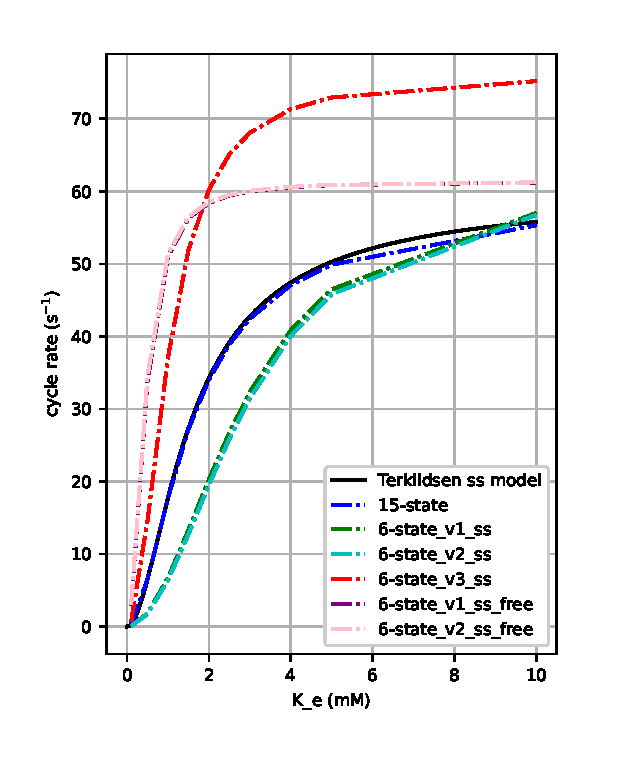
\includegraphics[width=\linewidth]{./figures/NKE_BG_6_state_fig3b_fit.eps}
            \caption{Fit to figure 3b of \cite{pan_cardiac_2020}.}
            \label{fig:fit_3b}
      \end{subfigure}
      \begin{subfigure}[b]{0.49\textwidth}
            \includegraphics[width=\linewidth]{./figures/NKE_BG_6_state_fig3c_fit.eps}
            \caption{Fit to figure 3c of \cite{pan_cardiac_2020}.}
            \label{fig:fit_3c}
      \end{subfigure}
\end{figure}

Notes:
\begin{itemize}
      \item I had tried time course fitting (to save fitting time), the results are worse so I didn’t include them in the above figures.
      6-state\_v3\_ss\_free is not included as well due to the poor fitting.
      \item “ss” means that we fitted the steady state data, “\_free” means no constraints on the thermodynamical parameters of the NKE states.
      \item In general, ss with the constraints fit the data better than the “free” ones.
      \item The constraints mainly affect the figures with potential $V_m$ and $K_e$.
      \item The voltage dependency (v1 vs v2) does not seem to affect the steady state. I will analyze their effect on the dynamics later.
      \item The separation of  unbind of Na and ADP steps (v1 and v2 separated them while  v3 combined them) seems to be critical.
      \item Another round of fitting with corrected constraints and broarder parameter bounds is ongoing.
\end{itemize}


\subsection*{Energy based analysis of models of \Gls{nka} and comparision}
The reduction of free energy available from ATP hydrolysis results in an accumulation of intracellular Na\textsuperscript{+} ions \cite{jansen2003energy},
while increase in intracellular Pi and decreases in intracellular pH and ATP were associated with ischemic conditions \cite{huang1984regulation}.

ATP concentration ranges from 1.92–7.47 mM with average of 4.4 mM \cite{greiner_intracellular_2021},
while the recent study showed lower diastolic cytosolic ATP levels (less than 1 mM) than previously estimated and fluctuations during excitation-contraction coupling \cite{rhana_fueling_2024}.

TODO:
\begin{itemize}
      \item Thermodynamic efficiency of the pump under different conditions (vary ATP, ADP, Pi, pH, Na, K, V)
      \item Compare the efficiency of different models
      \item Compare the dynamics of different models
      \item Compare the heat production of different models
\end{itemize}

\section*{Discussion}


\section*{Conclusion}

 

\section*{Author Contributions}

Author1 designed the research. Author2 carried out all simulations, analyzed the data. Author1 and Author2 wrote the article. 

\section*{Acknowledgments}



% Uncomment if using bibtex (default)
\bibliography{sample}

% Uncomment if using biblatex
% \printbibliography

\section*{Supplementary Material}

An online supplement to this article can be found by visiting BJ Online at \url{http://www.biophysj.org}.

\end{document}
